\documentclass{beamer}

%\usetheme{Singapore}
%\usetheme{Madrid}
\usetheme{simpledso}
\usepackage{lmodern}
\usepackage[scale=2]{ccicons}

% TODO: 
%   position adjustement
%   change colours
%
\usepackage{graphicx}  % Required for including images
\usepackage{fancybox}
%% for tikz
\usepackage{dtklogos}
\usepackage{tikz}
\usetikzlibrary{mindmap,shadows}
\usepackage{smartdiagram}
% restart numbering footnotes per page
\usepackage{perpage}
\MakePerPage{footnote}
% use nice itemlists ..
%\usepackage{enumitem, color, amssymb}
% customize captions
\usepackage{caption}
\captionsetup[figure]{font=footnotesize,labelfont=footnotesize,skip=0pt,belowskip=0pt}

% Watermark background (simple theme)
\setwatermark{
\includegraphics[height=8cm]{img/ntua.png}}

\newcommand\FourQuad[4]{
    \begin{minipage}[b][.45\textheight][t]{.50\textwidth}\centering#1\end{minipage}\hfill%
    \begin{minipage}[b][.45\textheight][t]{.50\textwidth}\centering#2\end{minipage}\\[0.9em]
    \begin{minipage}[b][.45\textheight][t]{.50\textwidth}\centering#3\end{minipage}\hfill
    \begin{minipage}[b][.45\textheight][t]{.50\textwidth}\centering#4\end{minipage}%
}

\setbeamerfont{caption}{size=\scriptsize}

%%  for pros and cons
\newenvironment{proenv}{\only{\setbeamercolor{local structure}{fg=green}}}{}
\newenvironment{conenv}{\only{\setbeamercolor{local structure}{fg=red}}}{}

\title{Planning DSO contribution to EUREF densification project.}
% \subtitle{Data, products and preliminary results}
% \date{\today}
\date{}
\author{X. Papanikolaou, D. Anastasiou, V. Zacharis, A. Marinou, E. Tita, and D. Paradissis}
\institute{National Technical University of Athens\\Dionysos Satellite Observatory\\\url{http://dionysos.survey.ntua.gr}}

\begin{document}

%%
%% TITLE PAGE
%%
\begin{frame}[plain]
\maketitle
\begin{block}{}
    \begin{center}
      \textbf{EUREF Analysis Centre Workshop}\\
    AIU Bern, Switzerland, October 14-15, 2015 \\
    \end{center}
\end{block}
\end{frame}

%%
%% TABLE OF CONTENTS
%%
\begin{frame}
    \frametitle{Table of Contents}
    \tableofcontents
\end{frame}

\section{Introduction}

\begin{frame}\frametitle{DSO Recent Activity}\framesubtitle{}

  Dionysos Satellite Observatory (DSO) and Higher Geodesy Laboratory of the 
  National Technical University of Athens, have developed an automated processing
  scheme to accommodate the routine analysis of all available continuous GNSS 
  stations in Greece.
  \\
  This daily analysis process, is implemented for the last two years, yielding 
  results which help us further understand the complicated tectonic setting of 
  Greece and nearby regions.
  \\
  Important results, include:
  \begin{itemize}
    \item the recent volcanic activity in \emph{Santorini} (e.g. \cite{papoutsis}),
    \item the 2014 \emph{Kefallonia} earthquakes (e.g. \cite{sarkefalonia}, \cite{sakkas})
  \end{itemize}
\end{frame}

\begin{frame}\frametitle{SEISMO Project}\framesubtitle{}
  In the framework of the SEISMO\footnote{South Aegean Geodynamic And Tsunami Monitoring Platform} Project, platform has been upgraded,
  to include:

  \begin{itemize}
    \item more GNSS stations, divided into sub-networks,
    \item manipulation, archiving \& dissemination of GNSS data files,
    \item new processing capabilities (e.g. GPS+GLONASS processing),
    \item automatic archiving and publishing of results (via a dedicated web-site),
    \item integration with \texttt{GSAC} (\cite{gsac}) and \texttt{MySQL} databases,
    \item new results and products
  \end{itemize}

  The platform was in practice re-designed \& re-implemented.

\end{frame}

% \begin{frame}\frametitle{Status}\framesubtitle{}
% \end{frame}

\section{Contribution to EUREF}

\begin{frame}\frametitle{Motivation}\framesubtitle{}
  Via our contribution to EUREF and interaction with its community, we hope to:
  \begin{itemize}
    \item expand \& modernize our research activity,
    \item contribute to the GNSS community,
    \item take part in ongoing/future projects,
    \item expand our knowlegdbase,
    \item improve our academic services (NTUA is a University)
  \end{itemize}
\end{frame}

\begin{frame}\frametitle{Velocity Field}\framesubtitle{}
 \begin{figure}
 \begin{center}
 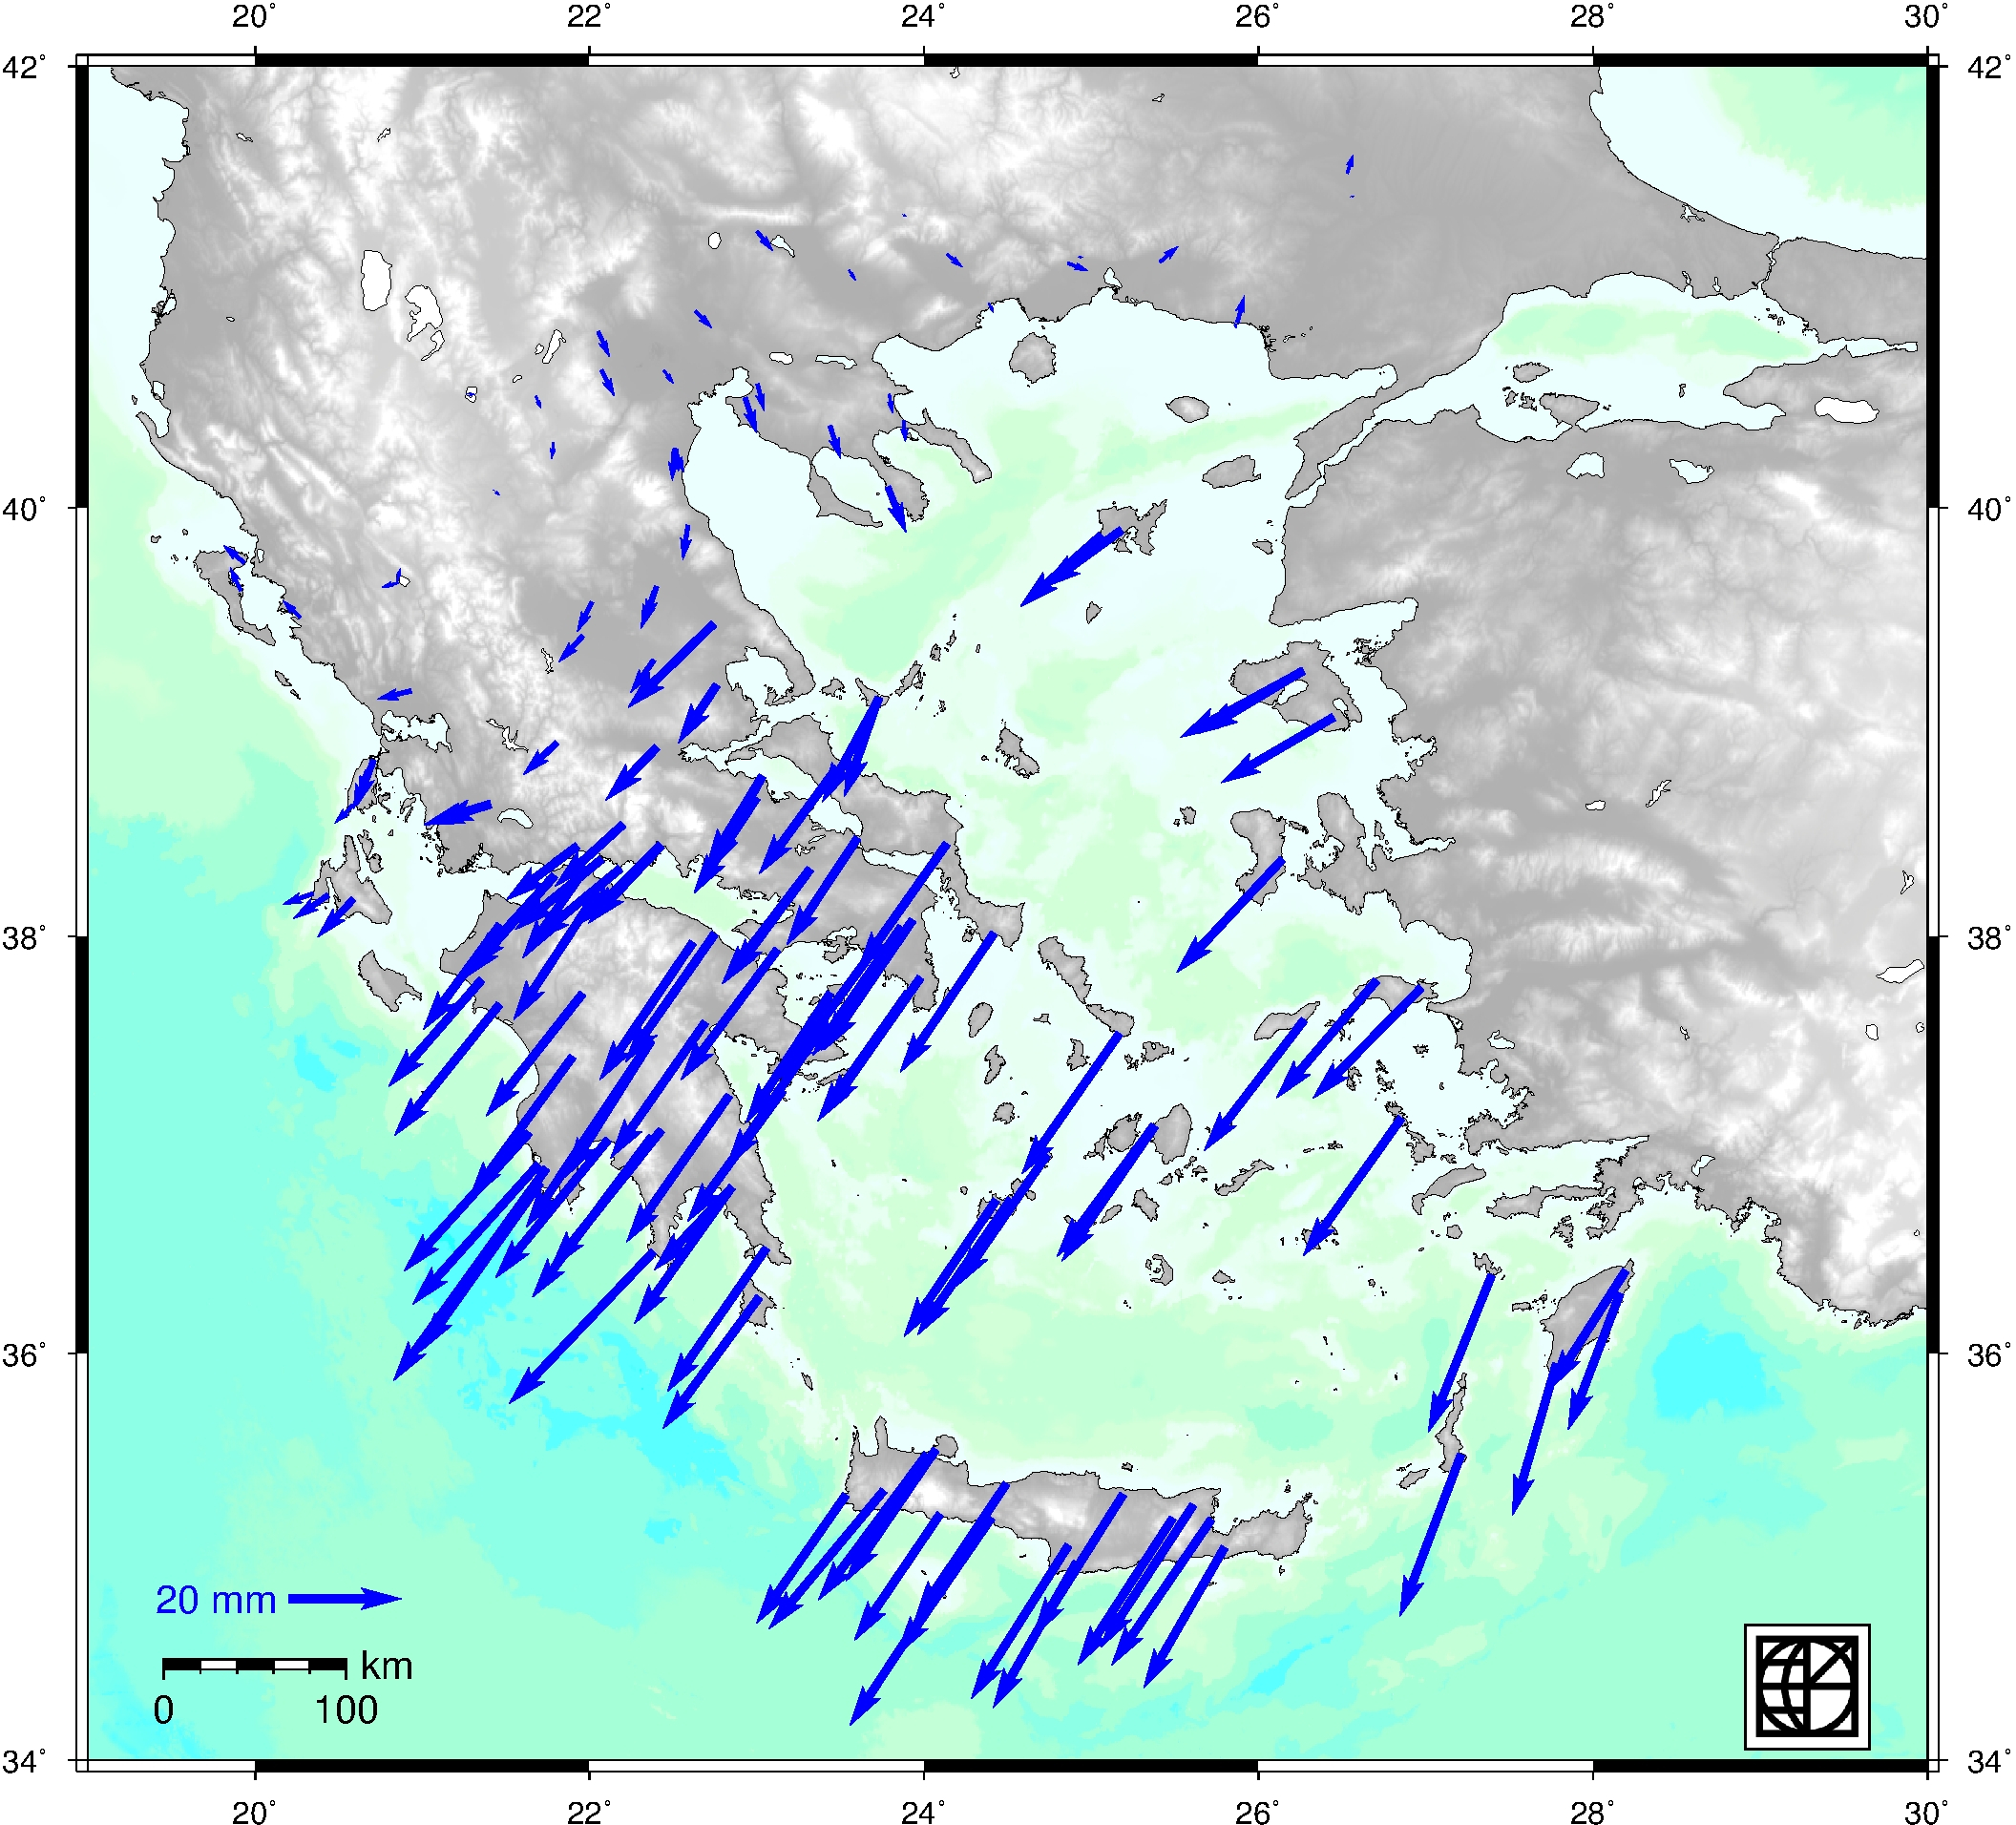
\includegraphics[width=.7\textwidth]{img/testvel.jpg}
 \caption{Velocity field in Greece wrt stable Europe \cite{papanikolaou}.}
 \label{fig:dgrm}
 \end{center}
 \end{figure}
\end{frame}

\section{GPS/GNSS Networks in Greece}

\begin{frame}\frametitle{Densification Network Selection}\framesubtitle{}
  To contribute to the Densification we have to establish a credible dataset
  (network). This has proven to be rather challenging !\\
  \bigskip
  Currently we process whatever we can get our hands on \ldots\\
  Problems:
  \begin{itemize}
    \item Inhomogenous dataset (\texttt{RINEX}, raw files, etc).
    \item Various maintainers, different mentalities.
    \item Different aquisition methods/rates.
    \item Hardly any log files.
    \item Wide variety of equipment (not always included in \texttt{atx} files).
  \end{itemize}
\end{frame}

\begin{frame}\frametitle{COMET/NTUA Network}\framesubtitle{}
%Network installed/maintained by \texttt{COMET}\footnote{Center for Observation and Modeling of Earthquakes, \url{http://comet.nerc.ac.uk/}} \& \texttt{NTUA}.
\begin{columns}[T] % align columns
\begin{column}{.40\textwidth}
  {\small
  \begin{itemize}
    \setlength\itemsep{.1em}
    \item<pro@1-> established along the Hellenic Arc
    \item<pro@1-> homogenous (geodetic type) equipment
    \item<pro@1-> credible time-span (early 2004 - late 2011)
    \item<con@1-> data aquisition stoped at late 2011
    \item<con@1-> equipment is old \& GPS-only
    \item<con@1-> needs repairing
\end{itemize}
}
\end{column}%
\hfill%
\begin{column}{.60\textwidth}
 \begin{figure}
 \begin{center}
 \vskip -.2cm
 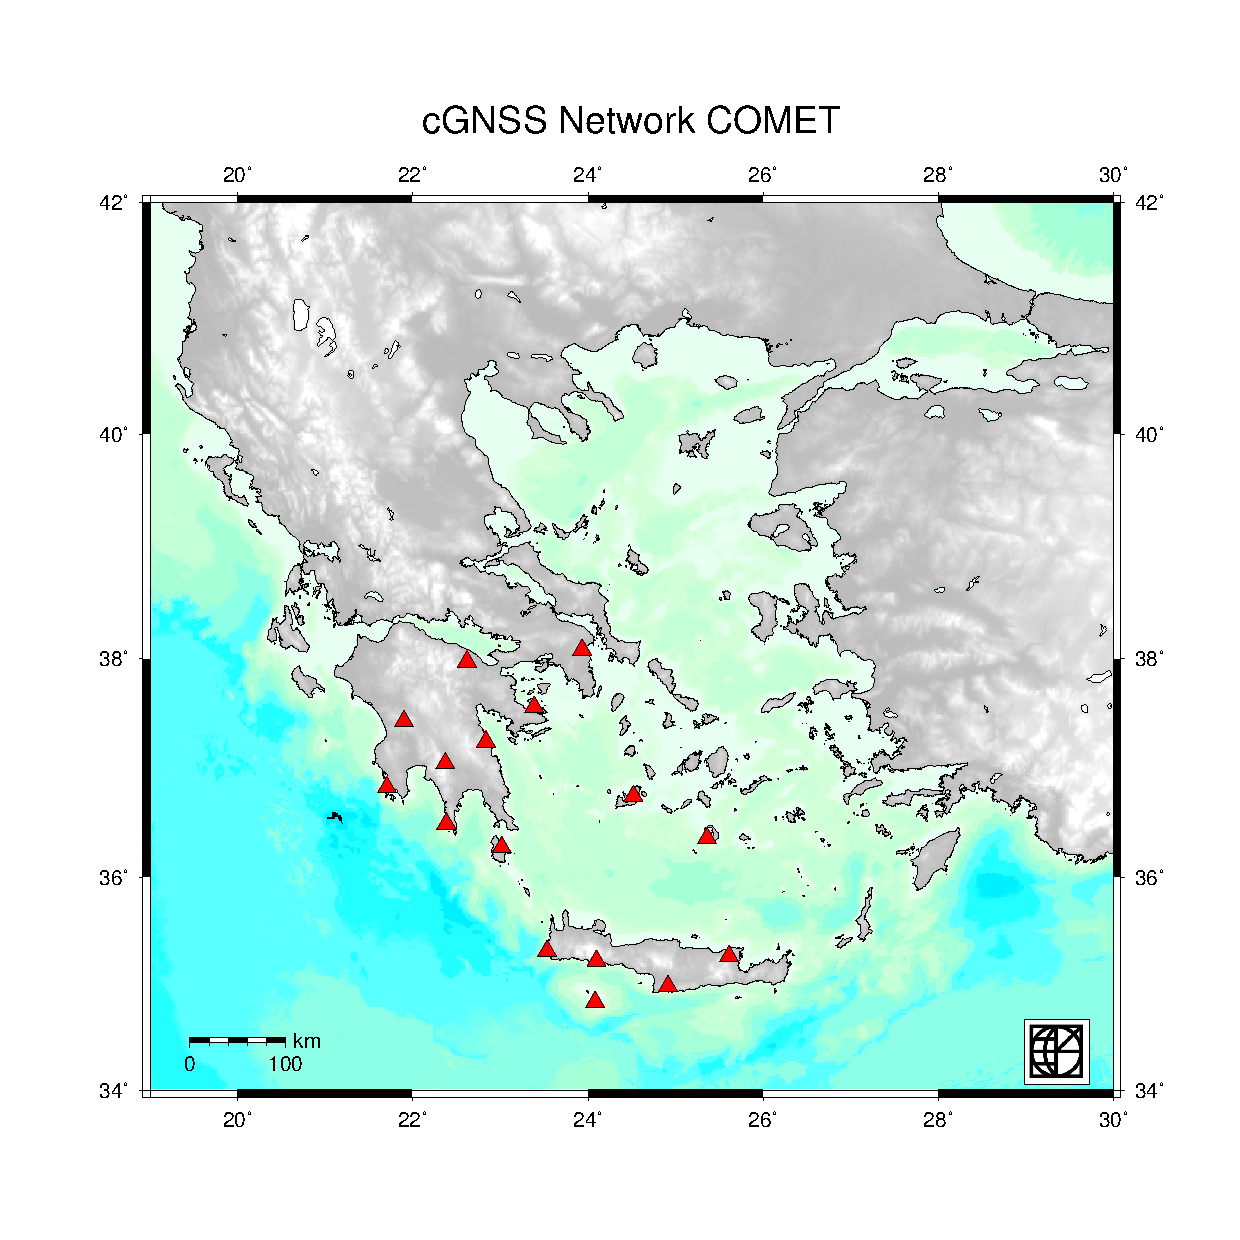
\includegraphics[trim={0cm 2.5cm 0cm 0cm},clip,width=.95\textwidth]{img/comet.eps} %1 2.2 0 0
 \vskip -.7cm
 \caption{COMET/NTUA network.}
 \label{fig:cometntua}
 \end{center}
 \end{figure}
\end{column}%
\end{columns}
  \begin{block}{}
    Can be used for EUREF densification ``as is''.
  \end{block}
\end{frame}

\begin{frame}\frametitle{NOA/GEIN and others}\framesubtitle{}
%Network maintained by \texttt{GEIN}/\texttt{NOA}\footnote{National Observatory of Athens \url{http://www.gein.noa.gr/services/GPS/noa\_gps.html}}. Sites established by various institutes
%(\texttt{NTUA, UNAVCO, MIT}).
\begin{columns}[T] % align columns
\begin{column}{.40\textwidth}
  \begin{itemize}
    \item<pro@1-> covers (sparsely) all of Greece 
    \item<pro@1-> credible time-span (newest stations at 2012)
    \item<con@1-> inconsistent providers (for some stations)
    \item<con@1-> no log files
  \end{itemize}
\end{column}%
\hfill%
\begin{column}{.60\textwidth}
 \begin{figure}
 \begin{center}
 \vskip -.2cm
 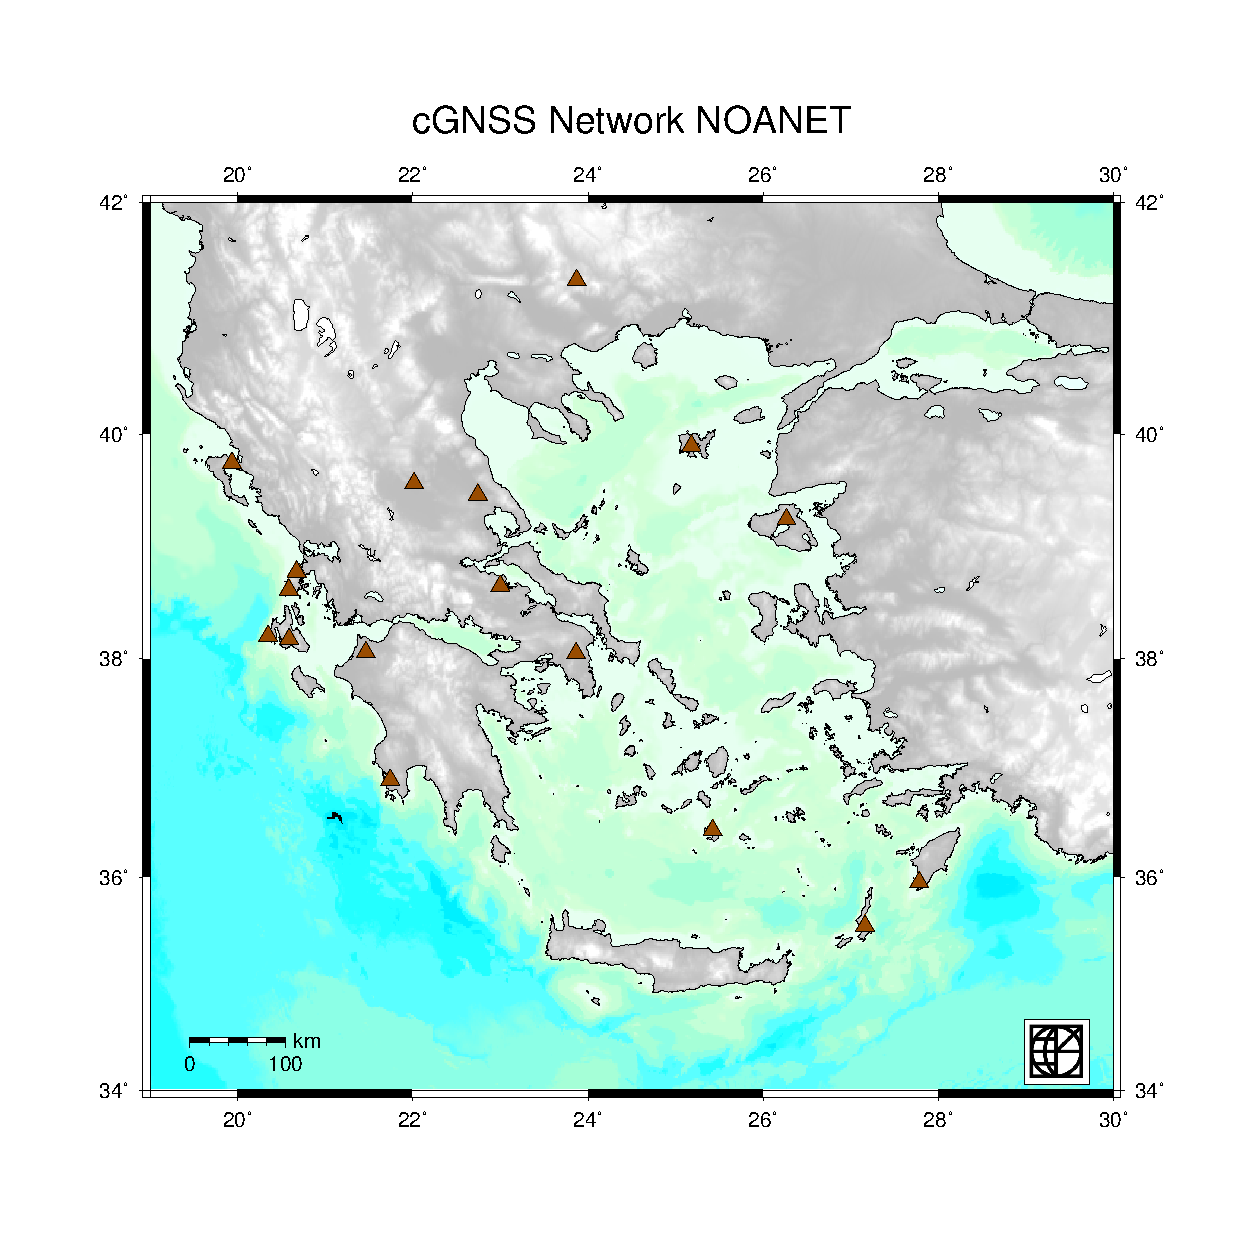
\includegraphics[trim={0cm 2.5cm 0cm 0cm},clip,width=.95\textwidth]{img/noanet.eps}
 \vskip -.7cm
 \caption{NOA/GEIN network.}
 \label{fig:noa}
 \end{center}
 \end{figure}
\end{column}%
\end{columns}
  \begin{block}{}
    Unusable sites: atal, stef (no calibration).
  \end{block}
\end{frame}

\begin{frame}\frametitle{Tree-Company / URANUS}\framesubtitle{}
%  Network installed/maintained by \texttt{Tree-Company}\footnote{URANUS network \url{http://www.uranus.gr/}}.
\begin{columns}[T] % align columns
\begin{column}{.35\textwidth}
{\small
  \begin{itemize}
    \item<pro@1-> dense network, covers all of Greece
    \item<pro@1-> homogenous (geodetic type) equipment
    \item<con@1-> limited time-span (late 2013 onwards)
    \item<con@1-> no log files
    \item<con@1-> comercial usage oriented
    \item<con@1-> $\sim$ 2 years of data lost !
  \end{itemize}
  }
\end{column}%
\hfill%
\begin{column}{.65\textwidth}
 \begin{figure}
 \begin{center}
 \vskip .5cm
 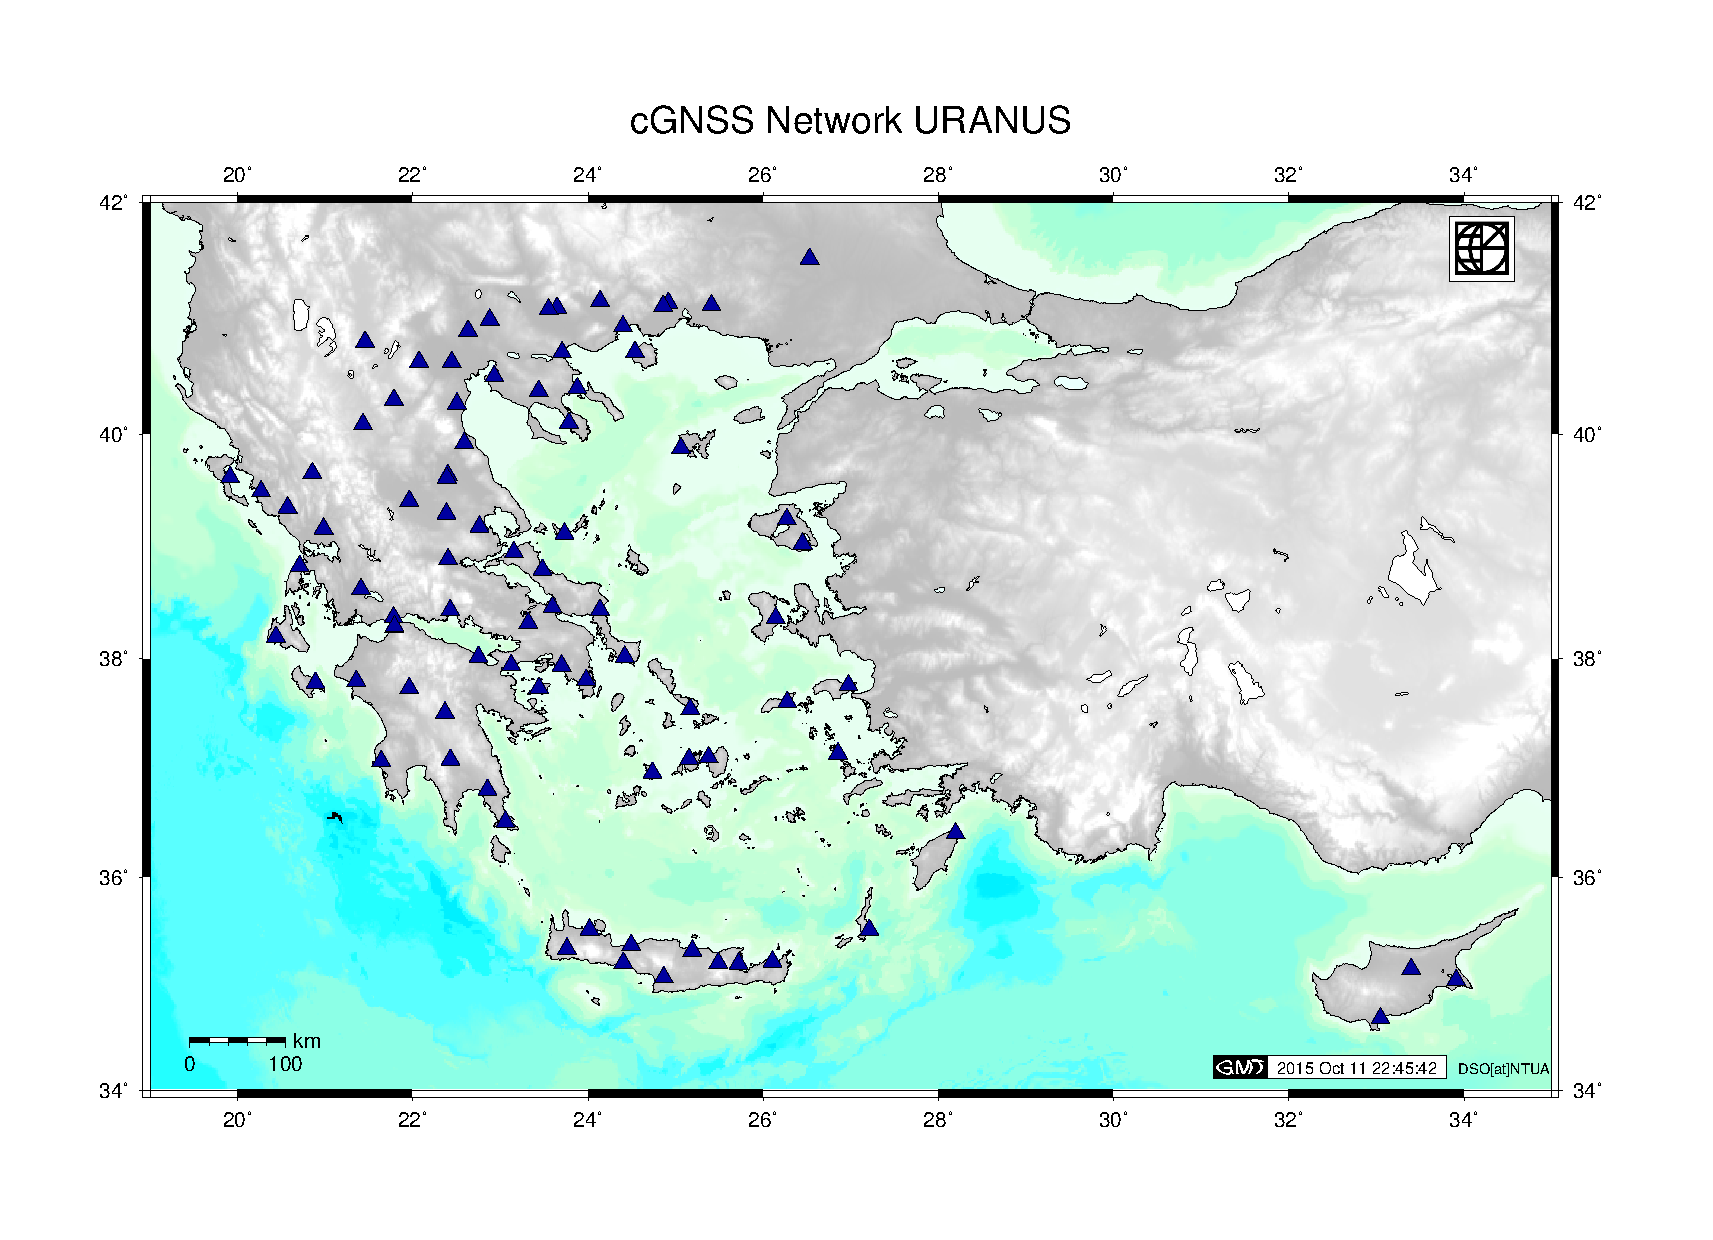
\includegraphics[trim={0cm 2.5cm 0cm 0cm},clip,width=1.1\textwidth]{img/uranus.eps}
 \vskip -.4cm
 \caption{Tree-Company URANUS network.}
 \label{fig:uranus}
 \end{center}
 \end{figure}
\end{column}%
\end{columns}
  \begin{block}{}
  Can only use sites with time-span > 2 years. 
  \end{block}
\end{frame}

\begin{frame}\frametitle{HEPOS}\framesubtitle{}
%  Network installed/maintained by \texttt{HEPOS}\footnote{\url{http://www.hepos.gr/}} (Greek Cadastre Service). 
\begin{columns}[T] % align columns
\begin{column}{.40\textwidth}
  \begin{itemize}
    \item<pro@1-> dense network, covers all of Greece
    \item<pro@1-> homogenous (geodetic type) equipment
    \item<con@1-> credible time-span (late 2007 onwards)
    \item<con@1-> limited access ($\sim$5 stations)!!
  \end{itemize}
\end{column}%
\hfill%
\begin{column}{.68\textwidth}
 \begin{figure}
 \begin{center}
 \vskip -.2cm
 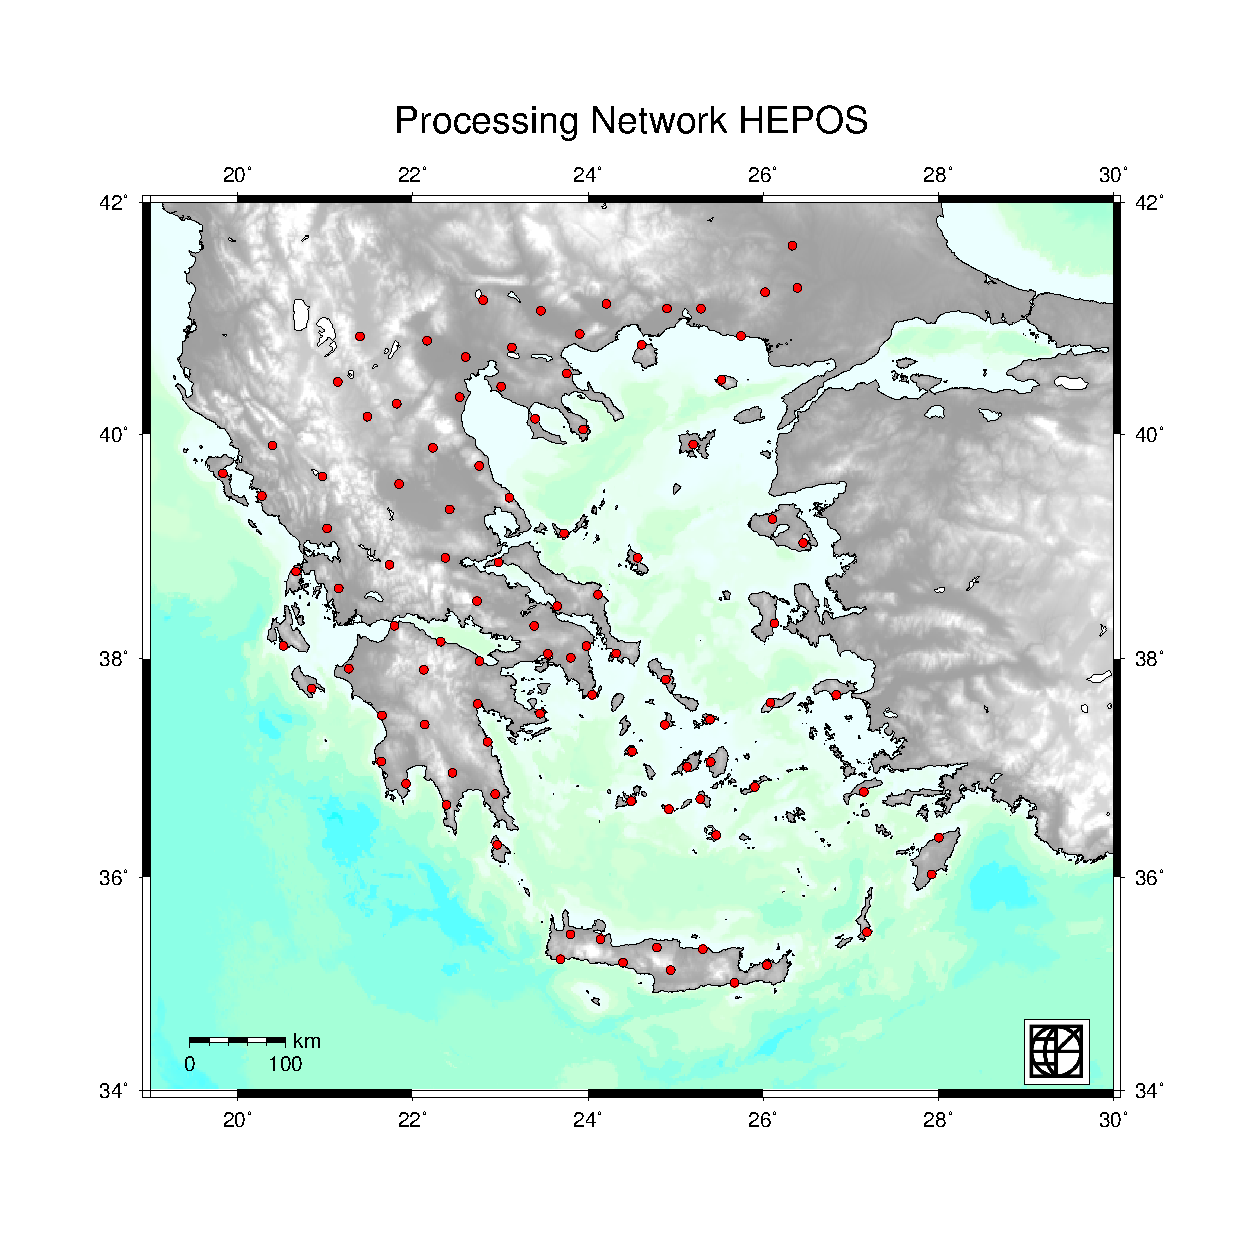
\includegraphics[trim={0cm 2.5cm 0cm 0cm},clip,width=.95\textwidth]{img/heposnet.eps}
 \vskip -.7cm
 \caption{HEPOS network.}
 \label{fig:hepos}
 \end{center}
 \end{figure}
\end{column}%
\end{columns}
  \begin{block}{}
  Can only use somewhere between 5 and 10 sites for a time-span of $\sim$ 4 years.
  \end{block}
\end{frame}

\begin{frame}\frametitle{Local Networks}\framesubtitle{}
  %Network installed/maintained by \texttt{CRLab}\footnote{Rift Laboratory \url{http://webobs.crlab.eu/}}. 
  \FourQuad
  {
  \textbf{Corinth Rift.}
  \begin{itemize}
    \item<pro@1-> credible time-span
    \item<pro@1-> only covers the Corinth Rift
    \item<con@1-> inconsistent providers
    \item<con@1-> no log files \& equipment changes
  \end{itemize}
  }
  {
 \begin{figure}
 \begin{center}
 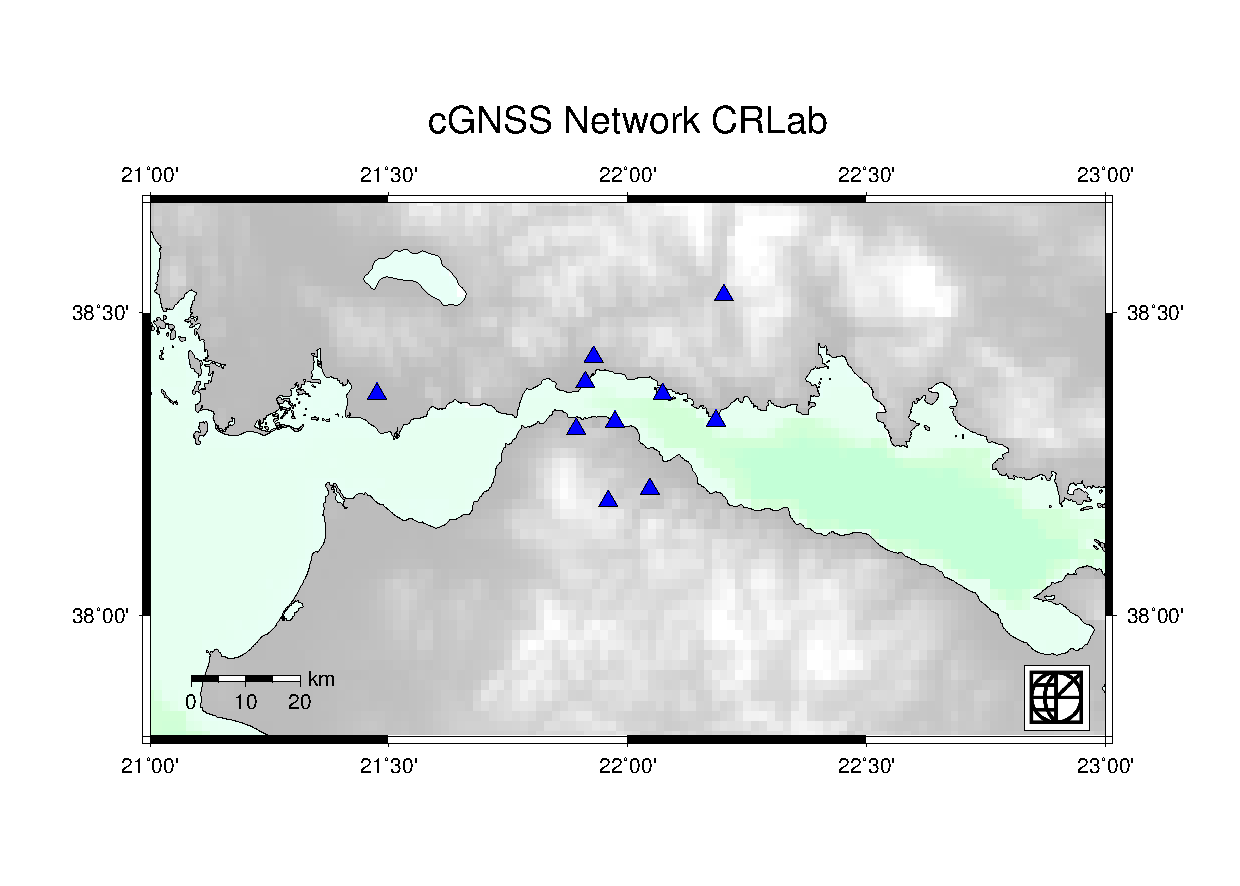
\includegraphics[trim={0cm 2.5cm 0cm 0cm},clip,width=.95\textwidth]{img/crlnet.eps}
  \vskip -.6cm
 \caption{CRLab network.}
 \label{fig:crlab}
 \end{center}
 \end{figure}
  }
  {
  \textbf{Santorini Network.}
  Most of the stations installed post-2011 to monitor the \textit{inflation episode}.
  \begin{itemize}
    \item<con@1-> localized
    \item<con@1-> limited time-span
  \end{itemize}
  }
  {
 \begin{figure}
 \begin{center}
 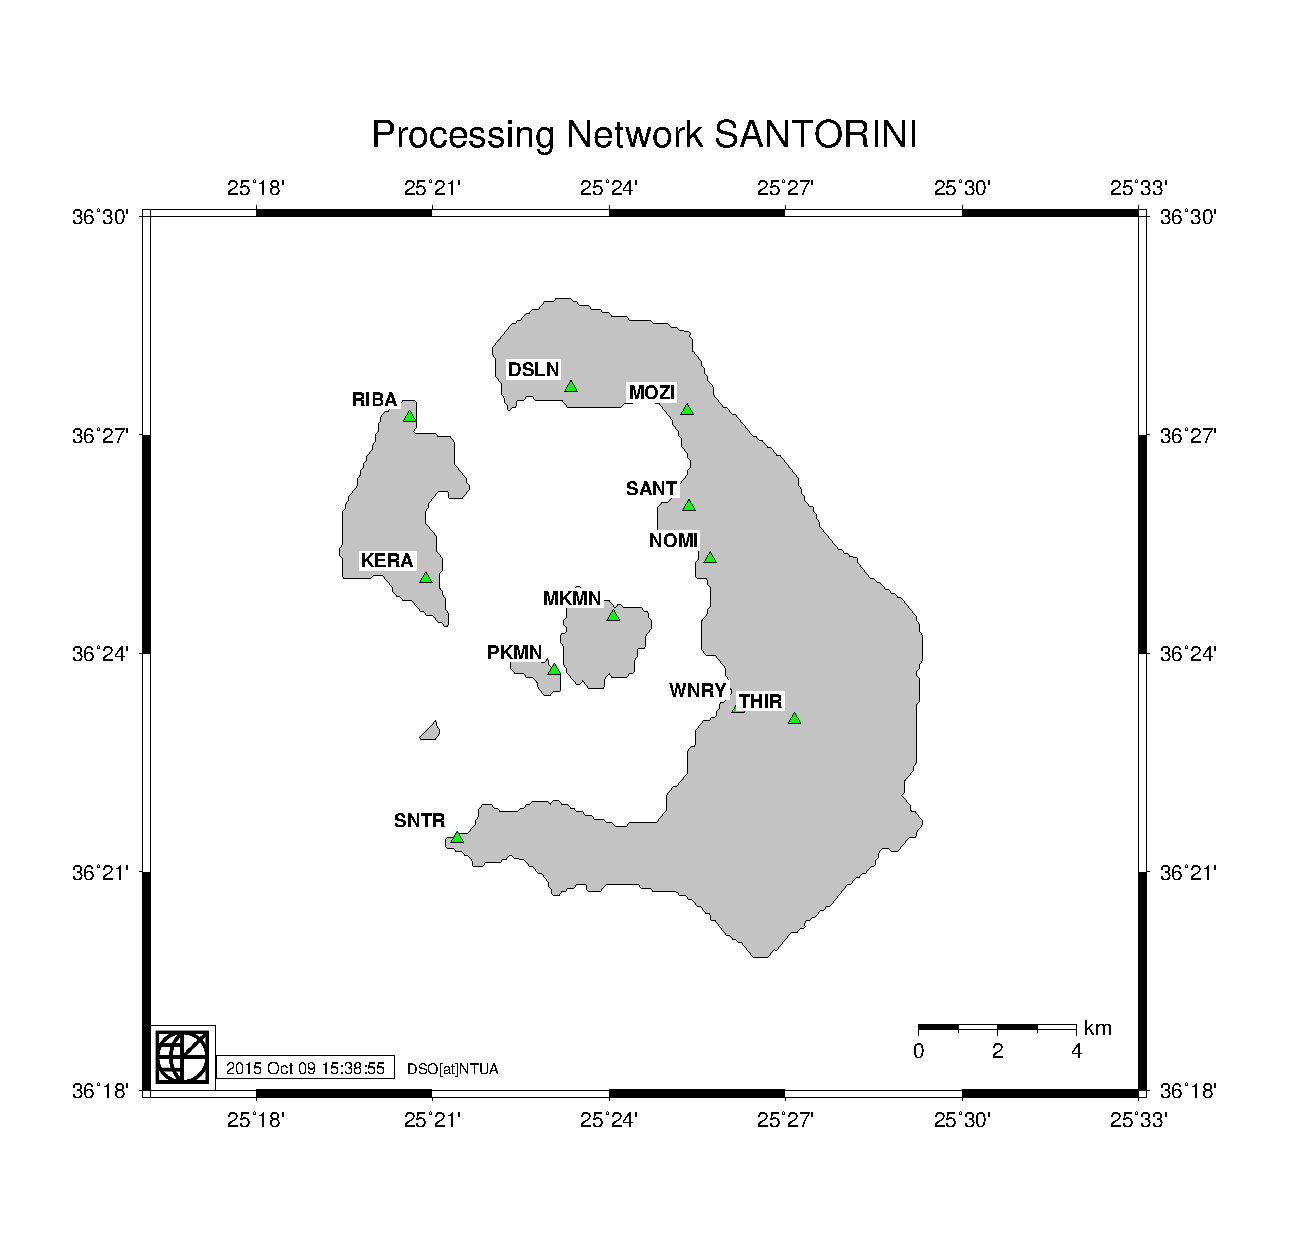
\includegraphics[trim={0cm 2.5cm 0cm 0cm},clip,width=.85\textwidth]{img/sntrnet.eps}
  \vskip -.6cm
 \caption{Santorini network.}
 \label{fig:sntrnet}
 \end{center}
 \end{figure}
  }
\end{frame}

\begin{frame}\frametitle{Densification Network}\framesubtitle{}
  The network to be used for the Densification, will look something like this \ldots
 \begin{figure}
 \begin{center}
 \vskip -.2cm
 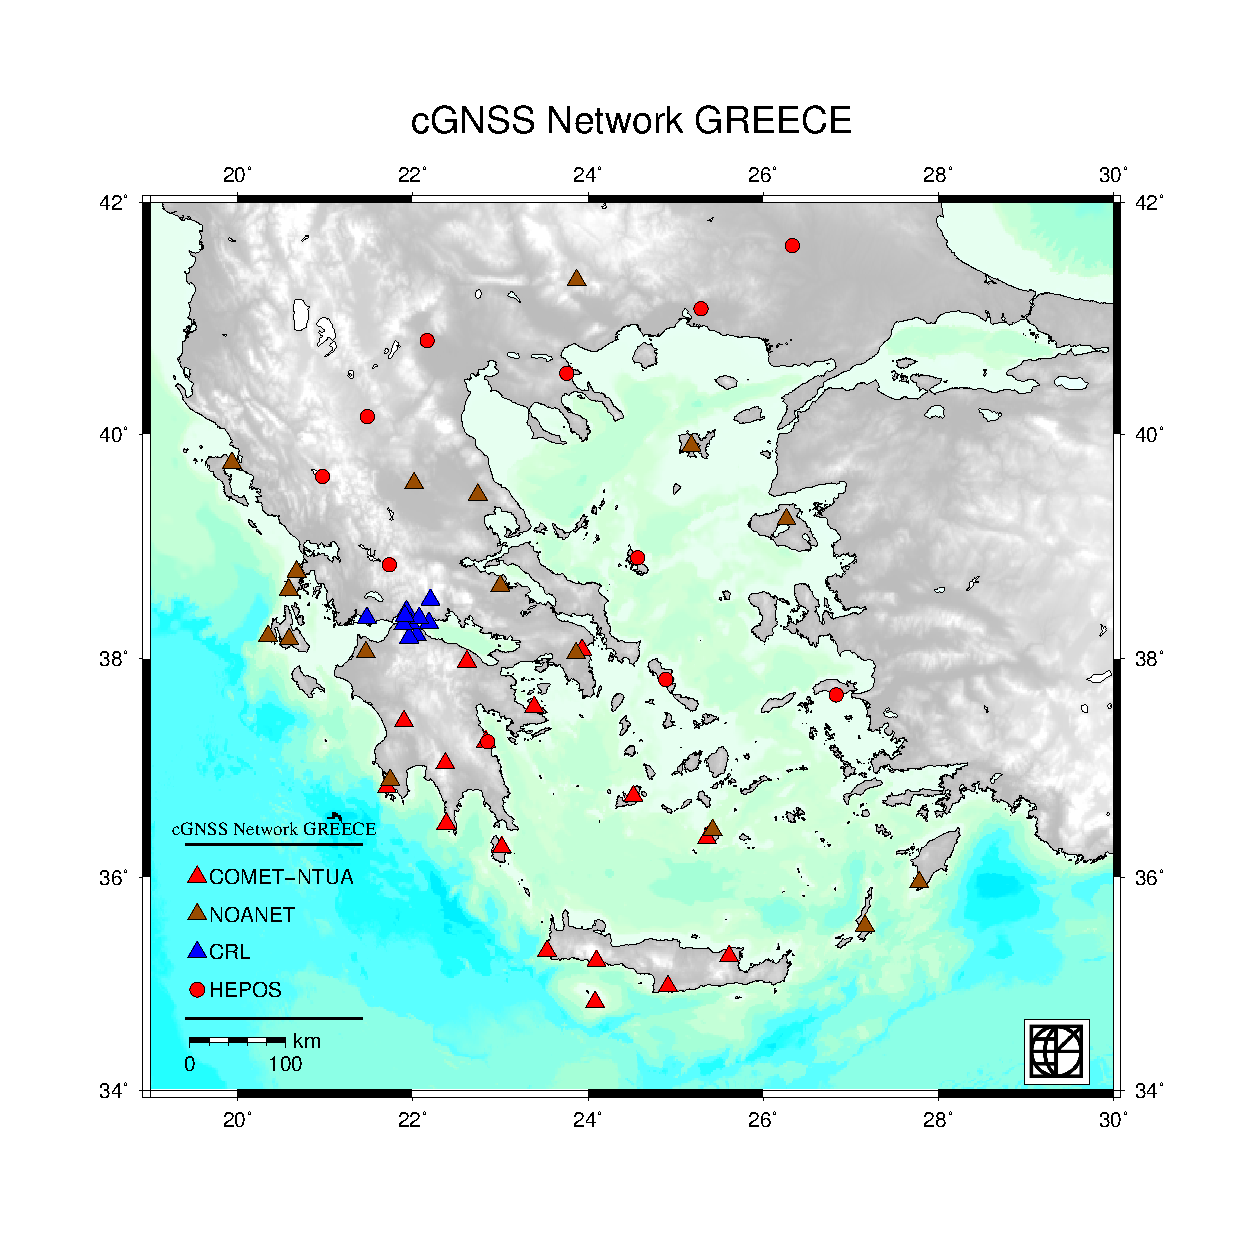
\includegraphics[trim={0cm 2.5cm 0cm 0cm},clip,width=.75\textwidth]{img/greeceall.eps}
  \vskip -.7cm
 \caption{Densification network (preliminary).}
 \label{fig:dgrm}
 \end{center}
 \end{figure}
\end{frame}

\section{Processing}

\begin{frame}\frametitle{The Scheme}\framesubtitle{}
\begin{columns}[T] % align columns
\begin{column}{.28\textwidth}
  The core tool/software is \texttt{Bernese GNSS Software v5.2}\cite{bpe}.\\
  \medskip
  Integration with 
  \begin{itemize}
    \item \texttt{MySQL} database,
    \item \texttt{Python} library
    \item \texttt{GSAC}
    \item wrappers (\texttt{shell})
  \end{itemize}
\end{column}%
\hfill%
\begin{column}{.68\textwidth}
\vskip -1cm
\begin{tikzpicture}[ every annotation/.style = {draw,
                     fill = white, font = \large}]

  \path[mindmap,concept color=black!40,text=white,
    every node/.style={concept,circular drop shadow, scale=.4},
    root/.style = {concept color=black!40,
      font=\normalsize\bfseries,text width=5em},
    level 1 concept/.append style={font=\normalsize\bfseries,
      sibling angle=50,text width=7.7em,
    level distance=20mm,inner sep=0pt},
    level 2 concept/.append style={font=\bfseries,level distance=15mm},
  ]

  node[root] {Bernese GNSS Software v5.2} [clockwise from=0]
    child[concept color=blue!60] {
      node {bernutils Python library} [clockwise from=90]
      child { node[concept] {github repo} }
      child { node[concept] {modules for Bernese output/control files} }
      child { node[concept] {modules for products} }
    }
    child[concept color=blue] {
      node[concept] {MySQL Database} [clockwise from=0]
      child { node[concept] {Bernese .STA} }
      child { node[concept] {IGS log files} }
      child { node[concept] {stations/networks/products} }
    }
    child[concept color=red] {
      node[concept] {/bin wrappers \& utils } [clockwise from=270]
      child { node[concept] {glue everything together} }
      child { node[concept] {various utilities \& formating} }
    }
    child[concept color=yellow!60!black] {
      node[concept] { GSAC } [clockwise from=220]
      child { node[concept] {RINEX} }
      child { node[concept] {products} }
    }
    child[concept color=green!40!black] {
      node[concept] { WebPage } [clockwise from=300]
    }
    \end{tikzpicture}
\end{column}%
\end{columns}
\end{frame}

\begin{frame}\frametitle{Compliance wrt EUREF standards}\framesubtitle{}
  Processing is consistent with EUREFF standards (\href{http://www.epncb.oma.be/_documentation/guidelines/guidelines_analysis_centres.pdf}{Guidelines for Analysis Centres}).
  \begin{itemize}%%[label={\checkmark}]
    \item \texttt{SINEX} with required info/blocks,
    \item Reference frame \texttt{IGb08},
    \item \texttt{IERS} Conventions 2010,
    \item \texttt{IGS}/\texttt{CODE} products,
    \item ocean loading corrections (\texttt{FES2004}),
    \item atmospheric tidal loading corrections,
    \item $3^{\circ}$ elevation cut-off angle; elevation dependent weighting,
    \item \texttt{GMF} and/or \texttt{VMF1}; \texttt{Chen-Herring} gradient parameter,
    \item amiguities fixed (length-dependent algorithm),
    \item use \texttt{GLONASS} obs (when available)
  \end{itemize}
\end{frame}

%  \begin{itemize}
%    \item check station information file consistency (against the provided in \texttt{CODE}'s ftp)
%    \item synchronize \texttt{GEN/} directory
%    \item closely follow \texttt{RNX2SNX.PCF}
%    \begin{itemize}
%      \item variabes in PCF are set by external tools (genericity)
%      \item skip copying/moving/removing; replace with tools that interconnect with \texttt{MySQL}
%    \end{itemize}
%    \item update database
%    \item customize output (\texttt{html, json})
%  \end{itemize}
% \end{frame}

\begin{frame}\frametitle{Workflow}\framesubtitle{}
\begin{columns}[T] % align columns
\begin{column}{.48\textwidth}
  \texttt{\$>ddproces.sh --year= --doy= --session= --bern-loadgps= --campaign= --satellite-system= --solution-id= --save-dir= --analysis-center= --use-ntua-products= --append-suffix= --elevation-angle= --update= --pcv= --apply-exclude-list}
\end{column}
\hfill%
\begin{column}{.48\textwidth}
  \scalebox{0.5}{
  \smartdiagram[priority descriptive diagram]{
    Download \texttt{RINEX} consulting \texttt{MySQL} db,
    Download products,
    Validate \texttt{.STA}; synchronize \texttt{/GEN},
    Set variables in the Protocol Control File (\texttt{.PCF}),
    Process the dataset,
    Check for errors,
    Save Products \& Update database records,
    Compile Report (\texttt{json} | \texttt{html})
}}
\end{column}
\end{columns}
\end{frame}

{
\usebackgroundtemplate{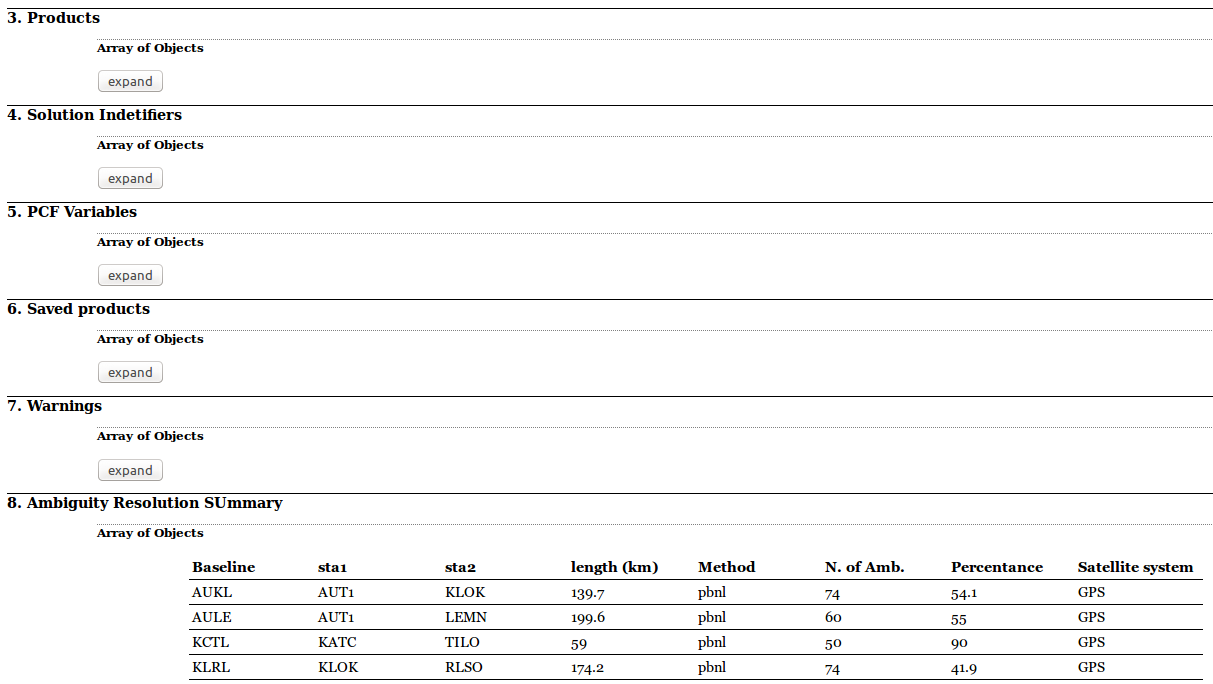
\includegraphics[height=.9\paperheight,width=.9\paperwidth]{img/jsonprint.png}}
\begin{frame}\frametitle{Results \& Output}\framesubtitle{}
\begin{center}
\vskip -1.6cm
\begin{tikzpicture}
  \node (img1) {\shadowbox{\color{black!35}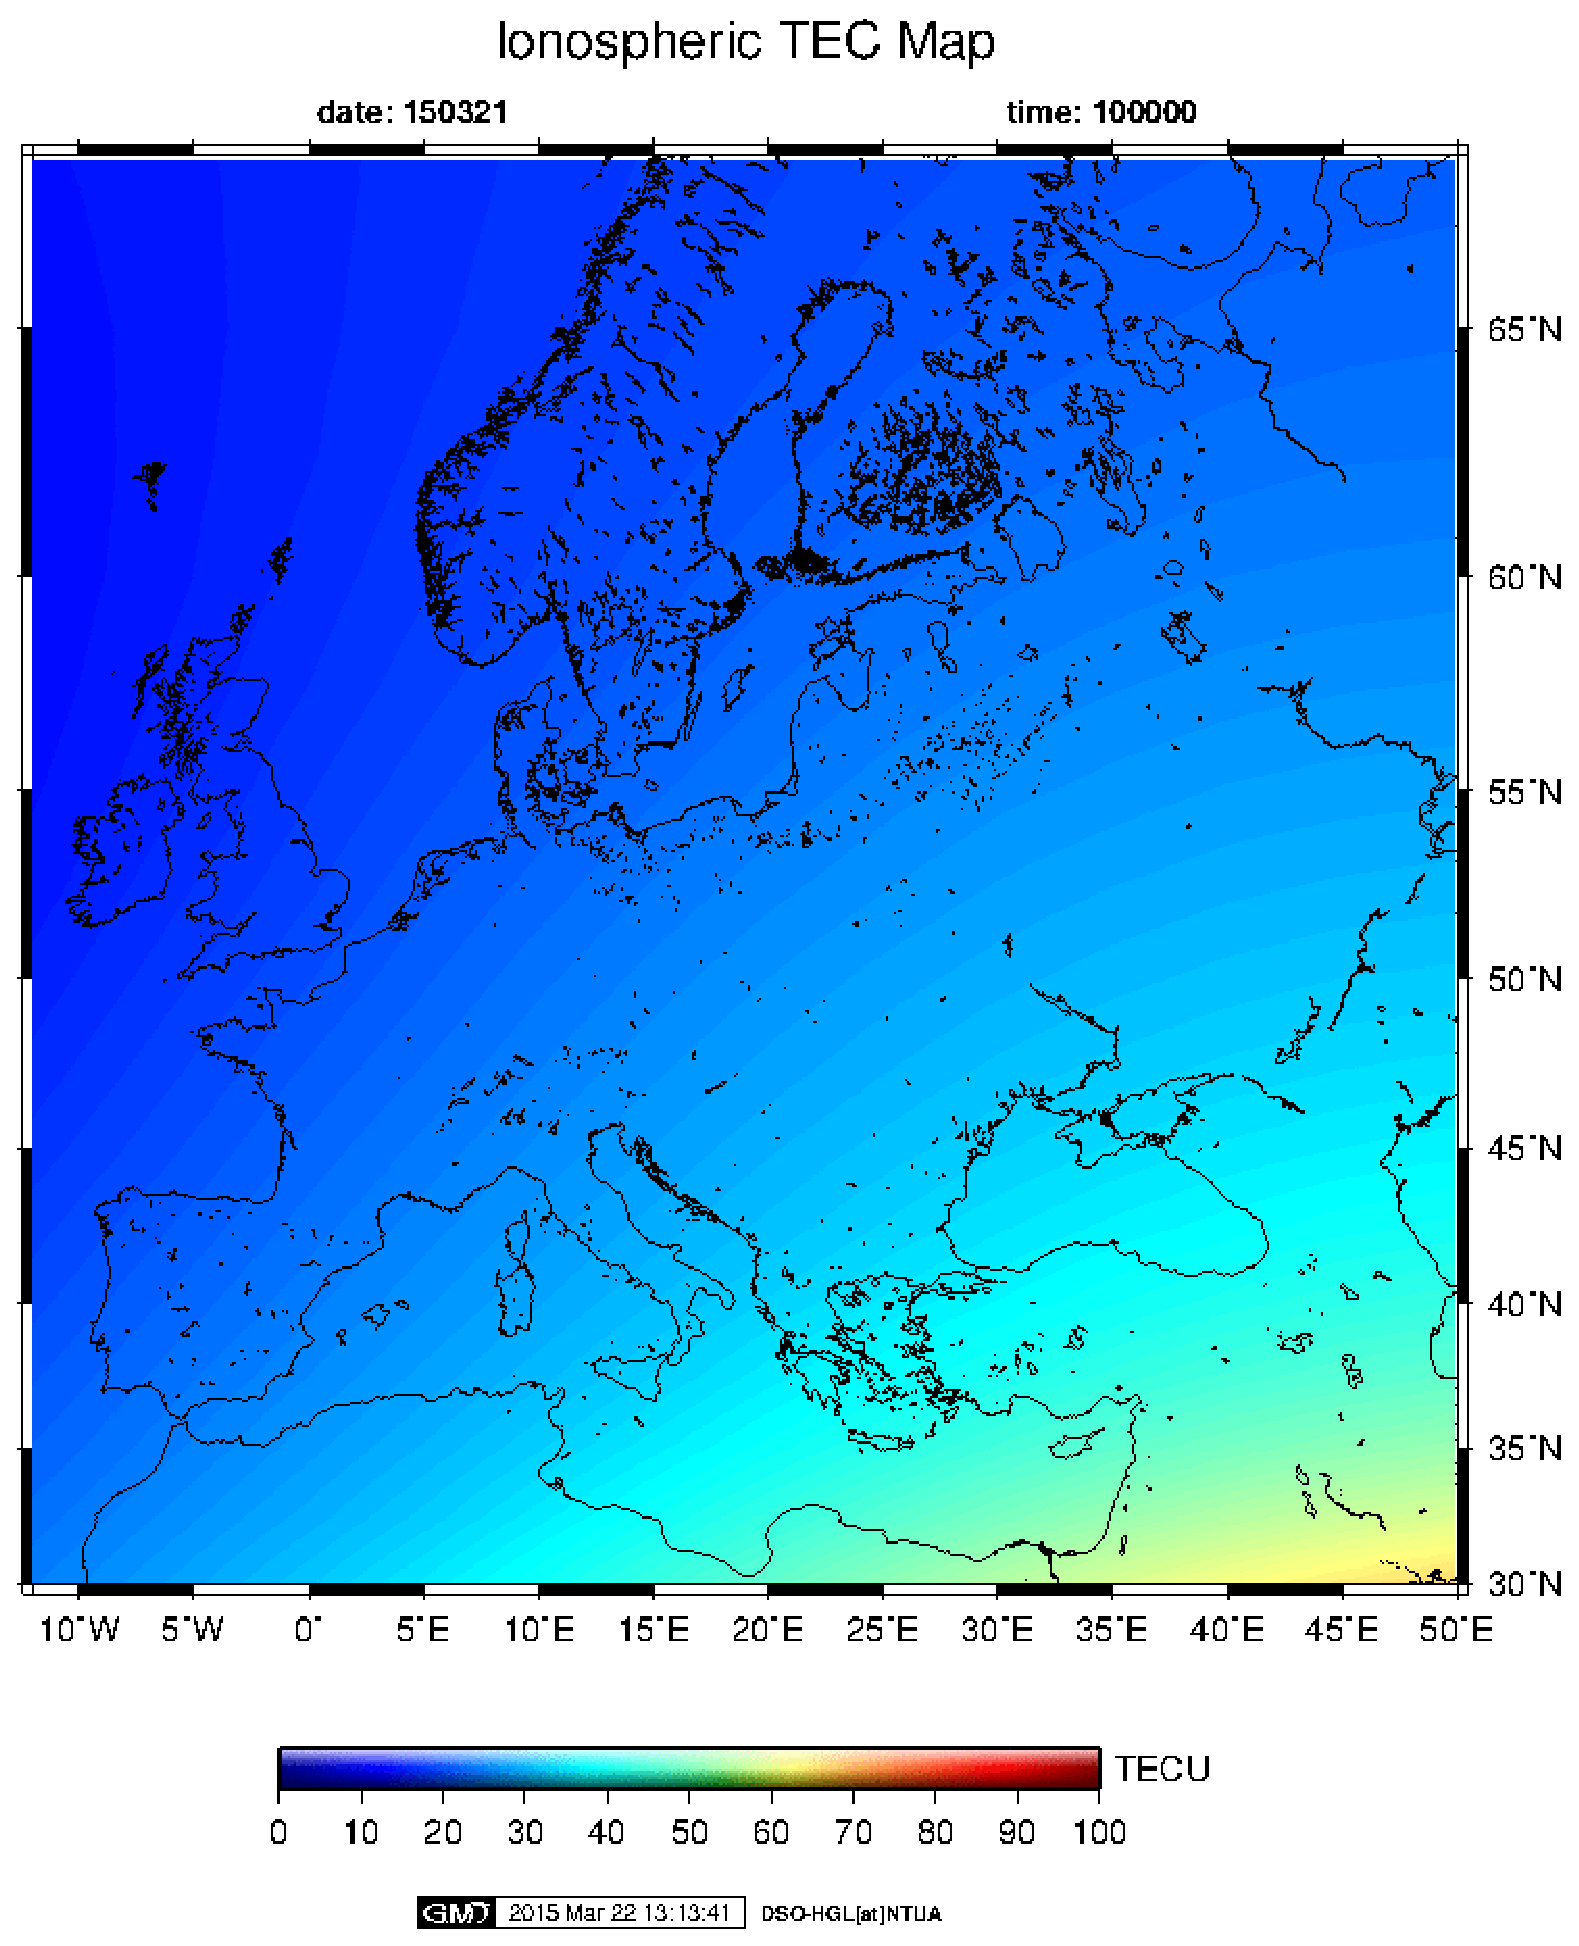
\includegraphics[height=4cm]{img/iono.eps}}};
%   \pause
  \node (img2) at (img1.north east) [yshift=-1cm,xshift=2.7cm] {\shadowbox{\color{black!35}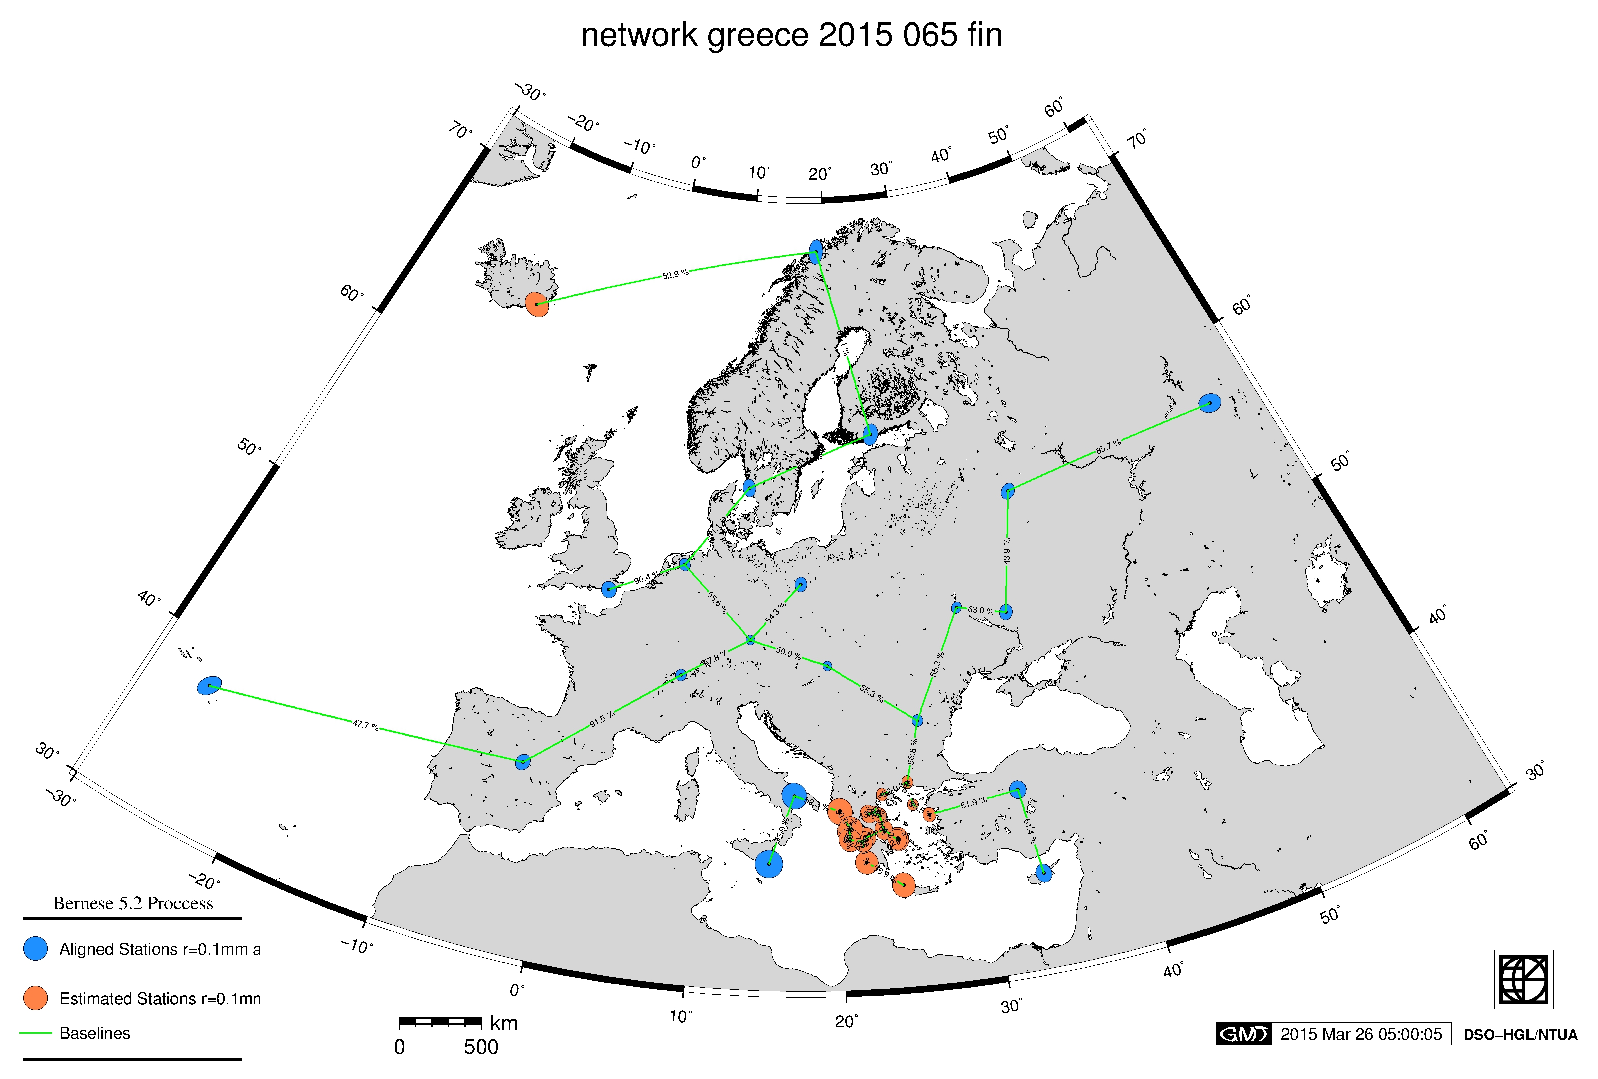
\includegraphics[height=2cm]{img/baseline.eps}}};
%   \pause
  \node (img3) at (img2.south) [yshift=-1.5cm,xshift=-.5cm] {\shadowbox{\color{black!35}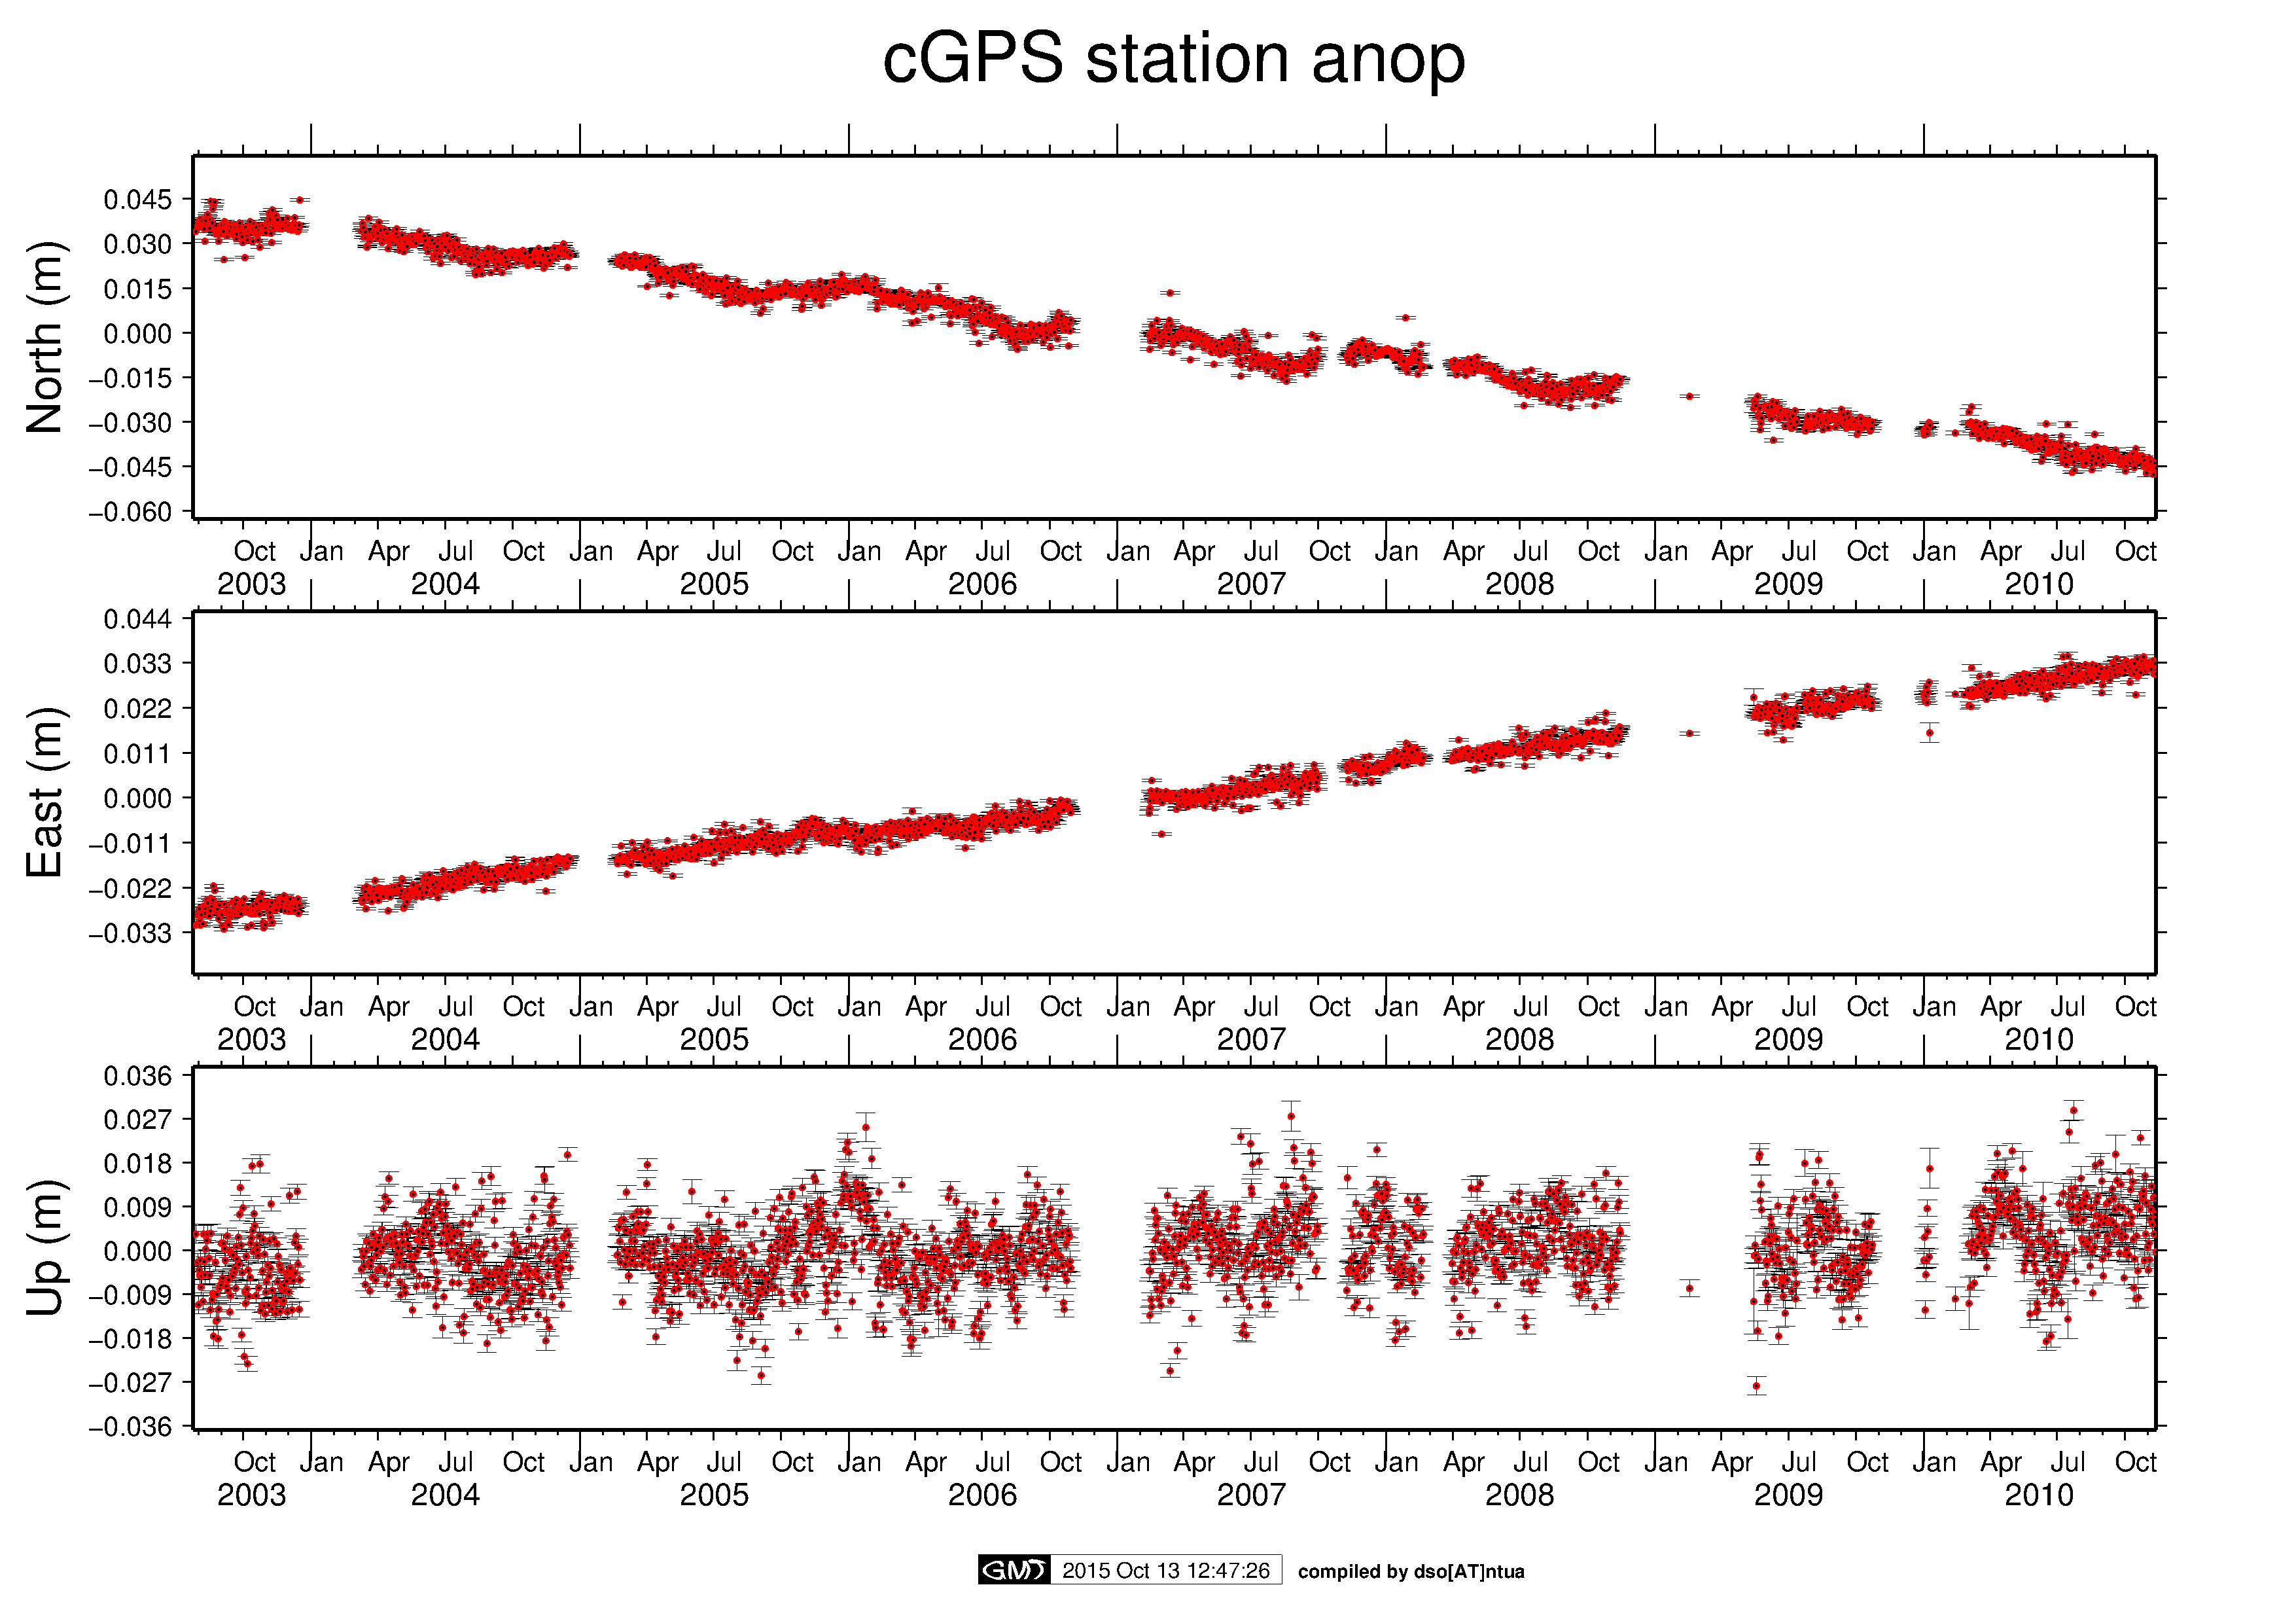
\includegraphics[height=2.6cm]{img/anop-raw.png}}};
%   \pause
%   \node (img4) at (img2.south west) [yshift=2cm] {\includegraphics[height=4cm]{img/dsoprint.png}};
\end{tikzpicture}
\end{center}
\end{frame}
}

\section{Web Resources}

\begin{frame}\frametitle{Web Resources}\framesubtitle{Visit, Browse, Interact, Comment}
\begin{itemize}
    \item \textbf{Dionysos Satellite Observatory} \url{http://dionysos.survey.ntua.gr/}  %%{http://dionysos.survey.ntua.gr/}
    \item \textbf{GSAC repository} \url{http://dionysos.survey.ntua.gr/dsoportal/_datacenter/gsacrepos.html} %%{http://dionysos.survey.ntua.gr/dsoportal/\_datacenter/gsacrepos.html}
    \item \textbf{Ftp site} \url{http://dionysos.survey.ntua.gr/dsoportal/_datacenter/ftpdata.html}  %%{http://dionysos.survey.ntua.gr/dsoportal/\_datacenter/ftpdata.html}
    \item \textbf{Kefallonia earthquake} \url{http://dionysos.survey.ntua.gr/dsoportal/_projects/supersites/cephalonia/}  %%{http://dionysos.survey.ntua.gr/dsoportal/\_projects/supersites/cephalonia/}
    \item \textbf{Ionospheric Remote Sensing} \url{http://dionysos.survey.ntua.gr/dsoportal/_projects/IonoRemSens/}  %%{}
\end{itemize}
\end{frame}

\section{Thank you}
\begin{frame}\frametitle{}\framesubtitle{}
    \begin{center}
    Thank you very much for your attention !
    \end{center}
\end{frame}

\begin{frame}[allowframebreaks]
  \frametitle<presentation>{References}
  \begin{thebibliography}{10}

%  \beamertemplatebookbibitems
%  \bibitem{Autor1990}
%    A.~Autor.
%    \newblock {\em Introduction to Giving Presentations}.
%    \newblock Klein-Verlag, 1990.

  \beamertemplatearticlebibitems

    %% Bernese
    \bibitem{bpe}
    Dach R., Hugentobler U., Fridez P., Meindl M.
    \newblock Bernese GPS Software Version 5.0
    \newblock {\em Astronomical Institute, University of Bern}, 2007.

    %% Papoutsis, Santorini
    \bibitem{papoutsis}
    Papoutsis I., Papanikolaou X., Floyd M., Ji K. H., Kontoes C., Paradissis D., Zacharis V.
    \newblock Mapping inflation at Santorini volcano, Greece, using GPS and InSAR
    \newblock {\em Geophysical Research Letters}, 40(2):267-272, 2013
    
    %% papanikolaou
    \bibitem{papanikolaou}
     X. Papanikolaou, D. Anastasiou, A. Marinou, V. Zacharis, and D. Paradissis 
    \newblock Routine Analysis of all available GNSS Stations in Greece: Data, products and preliminary results
    \newblock {\em  The Volcanic and Geodynamic Field of the South Aegean, International Workshop, 20-22 May, Santorini, Greece}


    %% Sakkas, Kephalonia
    \bibitem{sakkas}
    Sakkas V., Lagios E.
    \newblock Fault modelling of the early-2014 $\sim$ M6 Earthquakes in Cephalonia Island (W. Greece) based on GPS measurements
    \newblock {\em Tectonophysics}, Volumes 644–645,184-196, 2015, Pages 184-196

    %% Diaforoi, sar kephalonia
    \bibitem{sarkefalonia}
    Merryman Boncori J.P., Papoutsis I., Pezzo G., Tolomei C., Atzori S., Ganas A., Karastathis V., Salvi S., Kontoes C., Antonioli A.
    \newblock The February 2014 Cephalonia Earthquake (Greece): 3D Deformation Field and Source Modeling from Multiple SAR Techniques
    \newblock {\em Seismological Research Letters}, Vol.86(1), 2015

    %% Unavco GSAC
    \bibitem{gsac}
    UNAVCO
    \newblock GSAC -- Geodetic Seamless Archive Centers: Open-source Software for Geodesy Data Repositories
    \newblock {\em available at} \url{https://www.unavco.org/software/data-management/gsac/gsac.html}

    %% Unavco IGB08
    \bibitem{igb08}
    P. Rebischung
    \newblock IGb08: an update on IGS08
    \newblock {\em IGSMAIL [6663]} \url{http://igscb.jpl.nasa.gov/pipermail/igsmail/2012/007853.html}, 2012

    %% Unavco vmf1
    \bibitem{vmf1}
    Boehm J., B. Werl, and H. Schuh (2006)
    \newblock Troposphere mapping functions for GPS and very long baseline interferometry from European Centre for
    Medium-Range Weather Forecasts operational analysis data
    \newblock {\em Journal of Geophysical Research}, vol. 111, B02406, 2006

  \end{thebibliography}
\end{frame}

\end{document}
